\documentclass[a4paper,12pt]{article}
\usepackage[utf8]{vietnam}
\usepackage{hyperref}
\usepackage{graphicx}
\usepackage{xcolor}
\usepackage{subfigure}
\usepackage{float}
\usepackage{caption}
\usepackage{placeins}
\makeatletter
\setlength{\@fptop}{0pt}
\makeatother
\hypersetup{
	pdfborder = {0 0 0}
}
\title{\textbf{Báo cáo tuần 10 (P1) \\ Thực hành kiến trúc máy tính}}
\author{Họ tên: Phan Minh Anh Tuấn \\ MSSV: 20205227}
\date{}
\begin{document}
\maketitle
\tableofcontents
\newpage
\section{Assignment 1}
\subsection{Phân tích đề bài}
\textbf{Đề bài: }Create a new project, type in, and build the program of Home Assignment 1. Show different values on LED. \\
\textbf{MSSV: }20205227
$\rightarrow$ Cần hiển thị hai số 27
\FloatBarrier
\begin{figure}[ht!]
	\centerline{\fbox{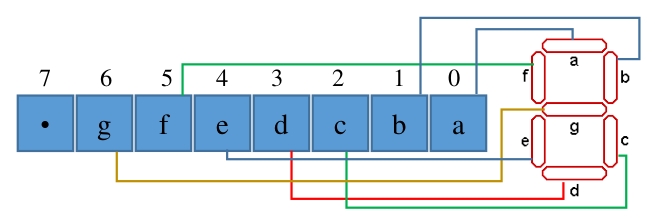
\includegraphics[width=1\textwidth]{ass1/number.png}}}
	\caption{Cấu trúc để hiện thị số LED 7 thanh}
	\label{fig:ass1}
\end{figure}
\noindent
\textbf{Hiển thị số 2}: Giá trị nhị phân là 11011011, giá trị hexa là 0xDF \\
\textbf{Hiển thị số 7}: Giá trị nhị phân là 10000111, giá trị hexa là 0x87 \\
\subsection{Triển khai MIPS}
\FloatBarrier
\begin{figure}[ht!]
	\centerline{\fbox{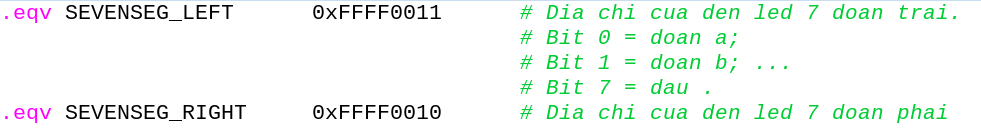
\includegraphics[width=1\textwidth]{ass1/address.png}}}
	\caption*{Bước 1: Truyền địa chỉ LED 7 thanh bên trái và bên phải}
	\label{fig:ass1}
\end{figure}
\FloatBarrier
\begin{figure}[ht!]
	\centerline{\fbox{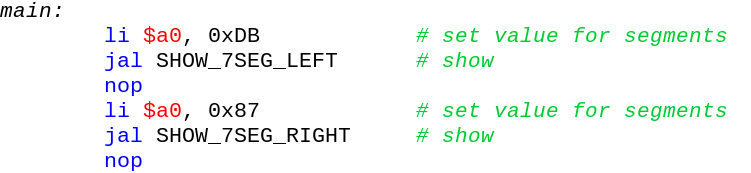
\includegraphics[width=1\textwidth]{ass1/main.png}}}
	\caption*{Bước 2: Truyền giá trị 0xDB, 0x87 vào \$a0 để hiện thị số trên LED 7 thanh}
	\label{fig:ass1}
\end{figure}
\FloatBarrier
\begin{figure}[ht!]
	\centerline{\fbox{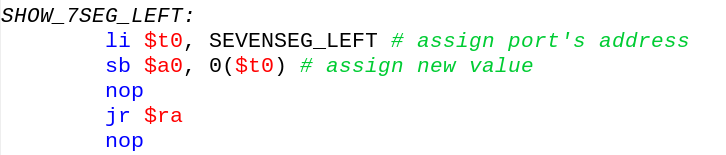
\includegraphics[width=1\textwidth]{ass1/show_left.png}}}
	\caption*{Bước 3: In giá trị của LED trái}
	\label{fig:ass1}
\end{figure}
\FloatBarrier
\begin{figure}[ht!]
	\centerline{\fbox{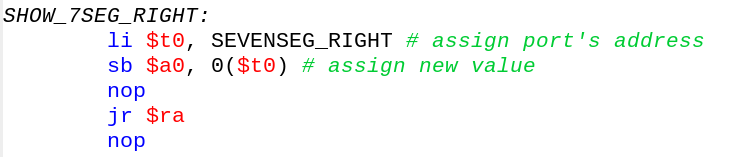
\includegraphics[width=1\textwidth]{ass1/show_right.png}}}
	\caption*{Bước 4: In giá trị của LED phải}
	\label{fig:ass1}
\end{figure}
\FloatBarrier
\begin{figure}[ht!]
	\centerline{\fbox{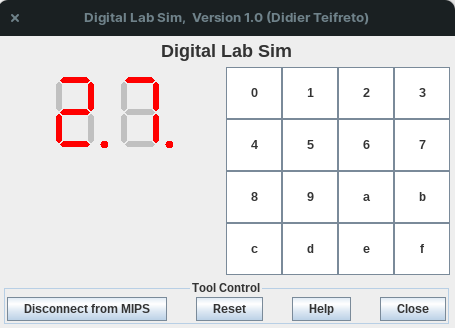
\includegraphics[width=1\textwidth]{ass1/result.png}}}
	\caption{Kết quả của đoạn code}
	\label{fig:ass1}
\end{figure}
\clearpage
\section{Assignment 2}
\textbf{Đề bài: }Create a new project, type in, and build the program of Home Assignment 2. Draw something.
\subsection{Triển khai MIPS}
Thực hiện vẽ trên bitmap display với các thông số như hình vẽ 
\FloatBarrier
\begin{figure}[ht!]
	\centerline{\fbox{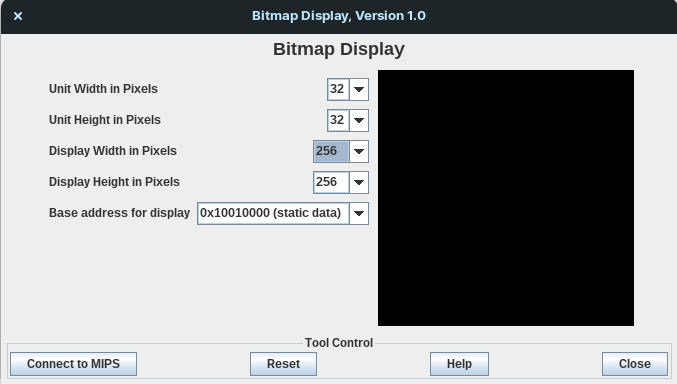
\includegraphics[width=1\textwidth]{ass2/demo.png}}}
	\caption{Các thông số của bitmap display}
	\label{fig:ass1}
\end{figure}
\FloatBarrier
\begin{figure}[ht!]
	\centerline{\fbox{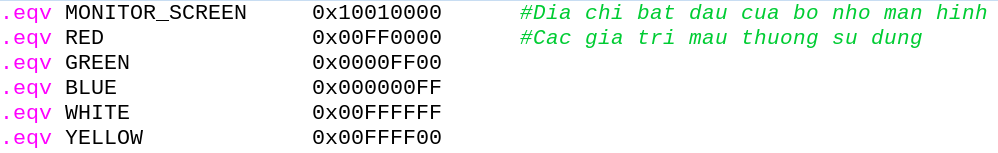
\includegraphics[width=1\textwidth]{ass2/init.png}}}
	\caption{Gán các địa chỉ của màn hình và màu sắc vào các biến}
	\label{fig:ass1}
\end{figure}
\FloatBarrier
\begin{figure}[ht!]
	\centerline{\fbox{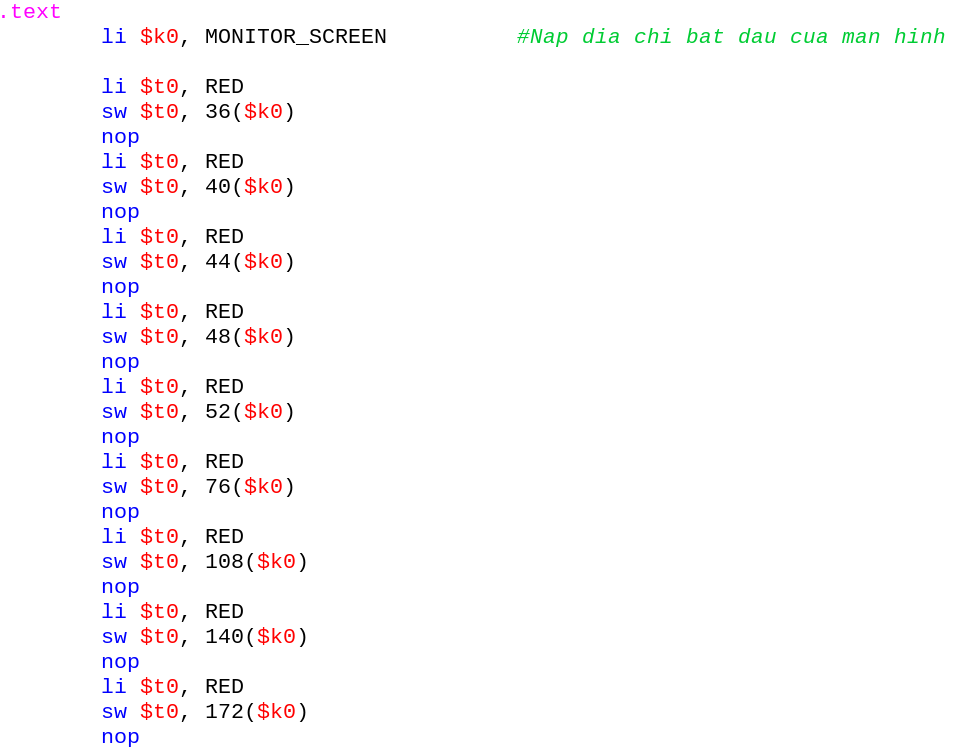
\includegraphics[width=1\textwidth]{ass2/drawT.png}}}
	\caption{Vẽ chữ T (thủ công)}
	\label{fig:ass1}
\end{figure}
\clearpage
\begin{figure}[ht!]
	\centerline{\fbox{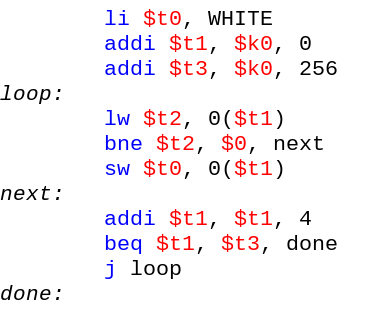
\includegraphics[width=0.6\textwidth]{ass2/drawW.png}}}
	\caption{Vẽ nền trắng}
	\label{fig:ass1}
\end{figure}
\noindent
\textbf{Giải thích: } \$t0 lưu giá trị của màu trắng, \$k0 lưu địa chỉ của màn hình. Với giá trị từ \$t1 đến \$t3, nếu địa chỉ tại ô đó chưa được tô trắng, thực hiện lệnh "sw \$t0, 0(\$t1)". Tăng giá trị của thanh ghi \$t1 và kiểm tra điều kiện lặp. 
\FloatBarrier
\begin{figure}[ht!]
	\centerline{\fbox{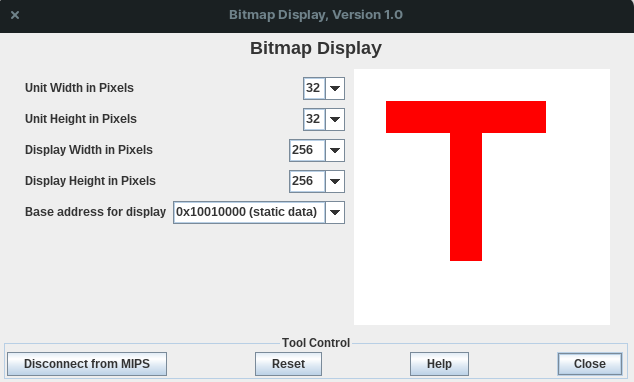
\includegraphics[width=1\textwidth]{ass2/result.png}}}
	\caption{Kết quả của đoạn code}
	\label{fig:ass1}
\end{figure}
\end{document}